\section{Back-propagation (12 pts)}

\subsection*{Introduction and Notation}

In this question, you will derive the necessary back-propagation operations for an efficient implementation of a feed-forward neural network for classification in Problem 6. Remember that the back-propagation algorithm calculates the gradient of each of the network's parameters to determine by how much to change them to achieve a better loss.\par

Let $f(x_1,x_2,x_3,\dots,x_n)=f(\bx)$ be a scalar output function of multiple scalar inputs, or a scalar output function of a single vector input. Recall the operator $\nabla$, defined as 
\begin{align}
    \nabla f = 
    \begin{bmatrix}
        \frac{\partial f}{\partial x_1}\\
        \cdots \\
        \frac{\partial f}{\partial x_n}
    \end{bmatrix}
\end{align}

In this homework, we will abuse the notation and extend $\nabla$. First let $W$ be a $r\times c$ matrix and $g(W)$ be a scalar output function. Define
\begin{align}
    \nabla_W [g] = 
    \begin{bmatrix}
        \frac{\partial g}{\partial W_{11}} & ... & \frac{\partial g}{\partial W_{1c}}\\
        \cdots & & \cdots\\
        \frac{\partial g}{\partial W_{r1}} & \cdots & \frac{\partial g}{\partial W_{rc}}
    \end{bmatrix}
\end{align}

(Note, this is not the Hessian, this is just a way to write and refer to each of the partial derivatives.) In addition, suppose $h(\bx,\by,W)$ is a scalar function of vectors $\bx$,$\by$, and a matrix W. Define 
\begin{align}
    \nabla_\bx [h] = 
    \begin{bmatrix}
        \frac{\partial h}{\partial x_1}\\
        \cdots \\
        \frac{\partial h}{\partial x_n}
    \end{bmatrix}
\end{align}
and similarly for $\nabla_\by [h]$ and $\nabla_W [h]$.

With these constructs at hand, let us derive back-propagation for a one hidden layer neural network with a softmax output and cross-entropy loss function. Let column vectors $\bx \in \R^D$ be a data-point and $\by \in \R^M$ be a one-hot encoding of the the corresponding label. Consider the neural network defined by the following equations.

\clearpage

\begin{figure}[h]
    \centering
    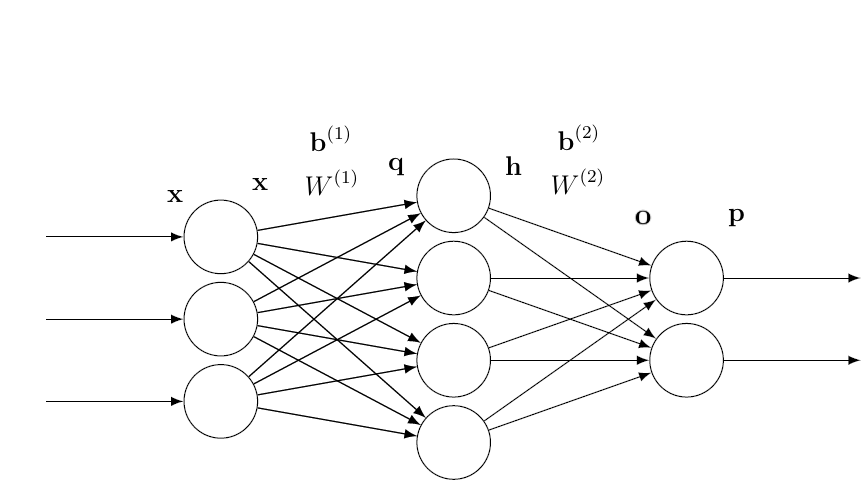
\includegraphics[width=0.9\textwidth]{images/neural-net.png}
    \caption{One layer fully connected neural network}
    \label{fig:my_label}
\end{figure}

\begin{align}
    \bq &= W^{(1)} \bx + \bb^{(1)} \\
    \bh &= \text{ReLU}(\bq)=\max{(0,\bq)} & \text{which is applied element-wise} \\
    \bo &= W^{(2)} \bh + \bb^{(2)} \\
    \bp &= \text{softmax}(\bo) & \text{which is defined as~}
    p_i = \frac{e^{o_i}}{\sum_{k=1}^M e^{o_k}} \\
    L(\bp, \by) &= - \sum_{i=1}^M y_i \log(p_i)
\end{align}

Note that $W^{(1)} \in \R^{H \times D}$, $\bb^{(1)} \in \R^H$, $W^{(2)} \in \R^{M \times H}$ and $\bb^{(2)} \in \R^M$.\par

Our ultimate goal is to calculate the gradients of the loss function with respect to the parameters $W^{(1)},\bb^{(1)},W^{(2)},\bb^{(2)}$. 

\clearpage


\subsection{(3 pts)}

In these sections, you may find it helpful to use the Kronecker delta (\url{https://en.wikipedia.org/wiki/Kronecker_delta}) as a shorthand. First, derive each of the following using chain rule:
\begin{align}
    \frac{\partial p_i}{\partial o_j},\ 
    \frac{\partial L}{\partial o_j},\ 
    \frac{\partial o_i}{\partial b_j^{(2)}},\ 
    \frac{\partial L}{\partial b_j^{(2)}}
\end{align}

\begin{soln}{height=10cm}
\ThreeAA
\end{soln}

Then, show that (by showing each element of the vectors are equal on both sides)
\begin{align}
    \nabla_\bo[L]=\bp - \by\\
    \nabla_{\bb^{(2)}}[L]=\bp - \by
\end{align}

\begin{soln}{height=5cm}
\ThreeAB
\end{soln}

\clearpage

\subsection{(3 pts)}

Derive the following using chain rule
\begin{align}
    \frac{\partial o_i}{\partial h_j},\ 
    \frac{\partial L}{\partial h_j}
\end{align}

\begin{soln}{height=11cm}
\ThreeBA
\end{soln}

Then, show that (by showing each element of the vectors are equal on both sides)
\begin{align}
    \nabla_{\bh} [L] &= W^{(2),\top}\nabla_{\bo}[L]
\end{align}
Note $W^{(2),\top}$ is the transpose of $W^{(2)}$\par

\begin{soln}{height=6cm}
\ThreeBB
\end{soln}

\clearpage

\subsection{(3 pts)}

Derive the following using chain rule
\begin{align}
    \frac{\partial o_k}{\partial W^{(2)}_{ij}},\ 
    \frac{\partial L}{\partial W^{(2)}_{ij}}
\end{align}

\begin{soln}{height=10cm}
\ThreeCA
\end{soln}

Then, show that (by showing each element of the matrices are equal on both sides) 
\begin{align}
    \nabla_{W^{(2)}} [L] = \nabla_\bo[L]\bh^{\top}
\end{align}

\begin{soln}{height=6cm}
\ThreeCB
\end{soln}

\clearpage

\subsection{(3 pts)}

Derive the following using chain rule. The second one should be in terms of $\frac{\partial L}{\partial h_i}$
\begin{align}
    \frac{\partial h_i}{\partial q_j},\ 
    \frac{\partial L}{\partial q_j}
\end{align}

\begin{soln}{height=12cm}
\ThreeD
\end{soln}

With these expressions at hand, you should be equipped to implement Problem $6$ efficiently. The derivative of $\bq$ with respect to $\bx$, $W^{(1)}$ and $\bb^{(1)}$ follows in the same way as $\bo$ with respect to $\bh$, $W^{(2)}$ and $\bb^{(2)}$.